\documentclass[11pt,a4paper]{article}

% Pakiety
\usepackage[utf8]{inputenc}
\usepackage[T1]{fontenc}
\usepackage[polish]{babel}
\usepackage{amsmath,amssymb,amsthm}
\usepackage{graphicx}
\usepackage{float}
\usepackage{booktabs}
\usepackage{hyperref}
\usepackage{geometry}
\usepackage{caption}
\usepackage{subcaption}
\usepackage{listings}
\usepackage{xcolor}

% Ustawienia strony
\geometry{margin=2.5cm}

% Styl kodu
\lstset{
    basicstyle=\ttfamily\small,
    breaklines=true,
    frame=single,
    language=Python,
    keywordstyle=\color{blue},
    commentstyle=\color{gray},
    stringstyle=\color{red}
}

% Definicje
\newtheorem{definition}{Definicja}
\newtheorem{theorem}{Twierdzenie}

\title{\textbf{Funkcje Interpolacji Fraktalnych}\\[0.5em]
\large Analiza funkcji Weierstrassa, krzywych wypełniających przestrzeń\\i fraktalnych funkcji interpolacyjnych}

\author{Projekt na przedmiot Fraktale}
\date{\today}

\begin{document}

\maketitle

\begin{abstract}
Niniejszy raport przedstawia implementację i analizę funkcji interpolacji fraktalnych. Zbadano funkcję Weierstrassa jako przykład funkcji ciągłej, wszędzie nieróżniczkowalnej, krzywe wypełniające przestrzeń (Hilberta, Peano) oraz fraktalne funkcje interpolacyjne (FIF). Do wyznaczania wymiaru fraktalnego zastosowano metodę box-counting (wymiar Minkowskiego). Wszystkie algorytmy zaimplementowano w języku Python i zweryfikowano na znanych przykładach.
\end{abstract}

\section{Wprowadzenie}

Fraktale to obiekty matematyczne charakteryzujące się \textbf{samopodobieństwem} -- ich struktura wygląda podobnie na różnych skalach. Kluczową właściwością fraktali jest ich \textbf{wymiar fraktalny}, który może przyjmować wartości niecałkowite.

W niniejszej pracy skupiamy się na trzech rodzajach funkcji fraktalnych:
\begin{enumerate}
    \item \textbf{Funkcja Weierstrassa} -- klasyczny przykład funkcji ciągłej, nigdzie nieróżniczkowalnej
    \item \textbf{Krzywe wypełniające przestrzeń} -- ciągłe krzywe przechodzące przez każdy punkt kwadratu
    \item \textbf{Fraktalne funkcje interpolacyjne (FIF)} -- metoda interpolacji z kontrolowaną strukturą fraktalną
\end{enumerate}

\section{Podstawy teoretyczne}

\subsection{Funkcja Weierstrassa}

\begin{definition}[Funkcja Weierstrassa]
Funkcja Weierstrassa jest zdefiniowana jako:
\begin{equation}
W(x) = \sum_{n=0}^{\infty} a^n \cos(b^n \pi x)
\end{equation}
gdzie $0 < a < 1$ i $b > 1$. Dla $ab > 1$ funkcja jest ciągła, ale nigdzie nieróżniczkowalna.
\end{definition}

\begin{theorem}[Wymiar fraktalny wykresu]
Dla funkcji Weierstrassa z parametrami $a$, $b$ spełniającymi $ab > 1$, wymiar Minkowskiego wykresu wynosi:
\begin{equation}
D = 2 + \frac{\log a}{\log b}
\end{equation}
\end{theorem}

Ponieważ $0 < a < 1$, mamy $\log a < 0$, więc $1 < D < 2$.

\subsection{Krzywe wypełniające przestrzeń}

Krzywe wypełniające przestrzeń (space-filling curves) to ciągłe krzywe, które przechodzą przez każdy punkt pewnego obszaru. Pierwszą taką krzywą skonstruował Giuseppe Peano w 1890 roku.

\textbf{Krzywa Hilberta} jest definiowana rekurencyjnie. Dla rzędu $n$:
\begin{itemize}
    \item Liczba punktów: $4^n$
    \item Długość segmentu: $2^{-n}$
    \item Całkowita długość: $L_n = 2^n \to \infty$
\end{itemize}

W granicy ($n \to \infty$) krzywa ma \textbf{wymiar fraktalny $D = 2$}.

\subsection{Wymiar Minkowskiego}

\begin{definition}[Wymiar Minkowskiego]
Dla zbioru $F$ w przestrzeni metrycznej:
\begin{equation}
\dim_{box}(F) = \lim_{\epsilon \to 0} \frac{\log N(\epsilon)}{\log(1/\epsilon)}
\end{equation}
gdzie $N(\epsilon)$ to minimalna liczba ``pudełek'' o rozmiarze $\epsilon$ potrzebna do pokrycia zbioru $F$.
\end{definition}

\textbf{Algorytm box-counting} (numeryczny):
\begin{enumerate}
    \item Dla różnych wartości $\epsilon$, oblicz $N(\epsilon)$
    \item Dopasuj prostą do punktów $(\log(1/\epsilon), \log N(\epsilon))$
    \item Wymiar = nachylenie prostej
\end{enumerate}

\subsection{Fraktalne funkcje interpolacyjne}

Fraktalne funkcje interpolacyjne (FIF) są konstruowane przy użyciu Iterated Function Systems (IFS). Dla punktów interpolacji $(x_0, y_0), \ldots, (x_n, y_n)$ i współczynników skalowania $d_1, \ldots, d_{n-1}$, wymiar FIF jest rozwiązaniem równania:
\begin{equation}
\sum_{i=1}^{n-1} |d_i|^D = 1
\end{equation}

Dla jednakowych współczynników $d_i = d$:
\begin{equation}
D = \frac{-\log(n-1)}{\log|d|}
\end{equation}

\section{Implementacja}

Wszystkie algorytmy zaimplementowano w języku Python z wykorzystaniem bibliotek NumPy, SciPy i Matplotlib. Struktura projektu:

\begin{itemize}
    \item \texttt{src/weierstrass.py} -- funkcja Weierstrassa
    \item \texttt{src/space\_filling.py} -- krzywe Hilberta, Peano, Dragon
    \item \texttt{src/box\_counting.py} -- algorytm wymiaru Minkowskiego
    \item \texttt{src/fractal\_interpolation.py} -- FIF
\end{itemize}

Kod został przetestowany zestawem 60 testów jednostkowych, wszystkie przechodzą pomyślnie.

\section{Wyniki}

\subsection{Funkcja Weierstrassa}

\begin{figure}[H]
    \centering
    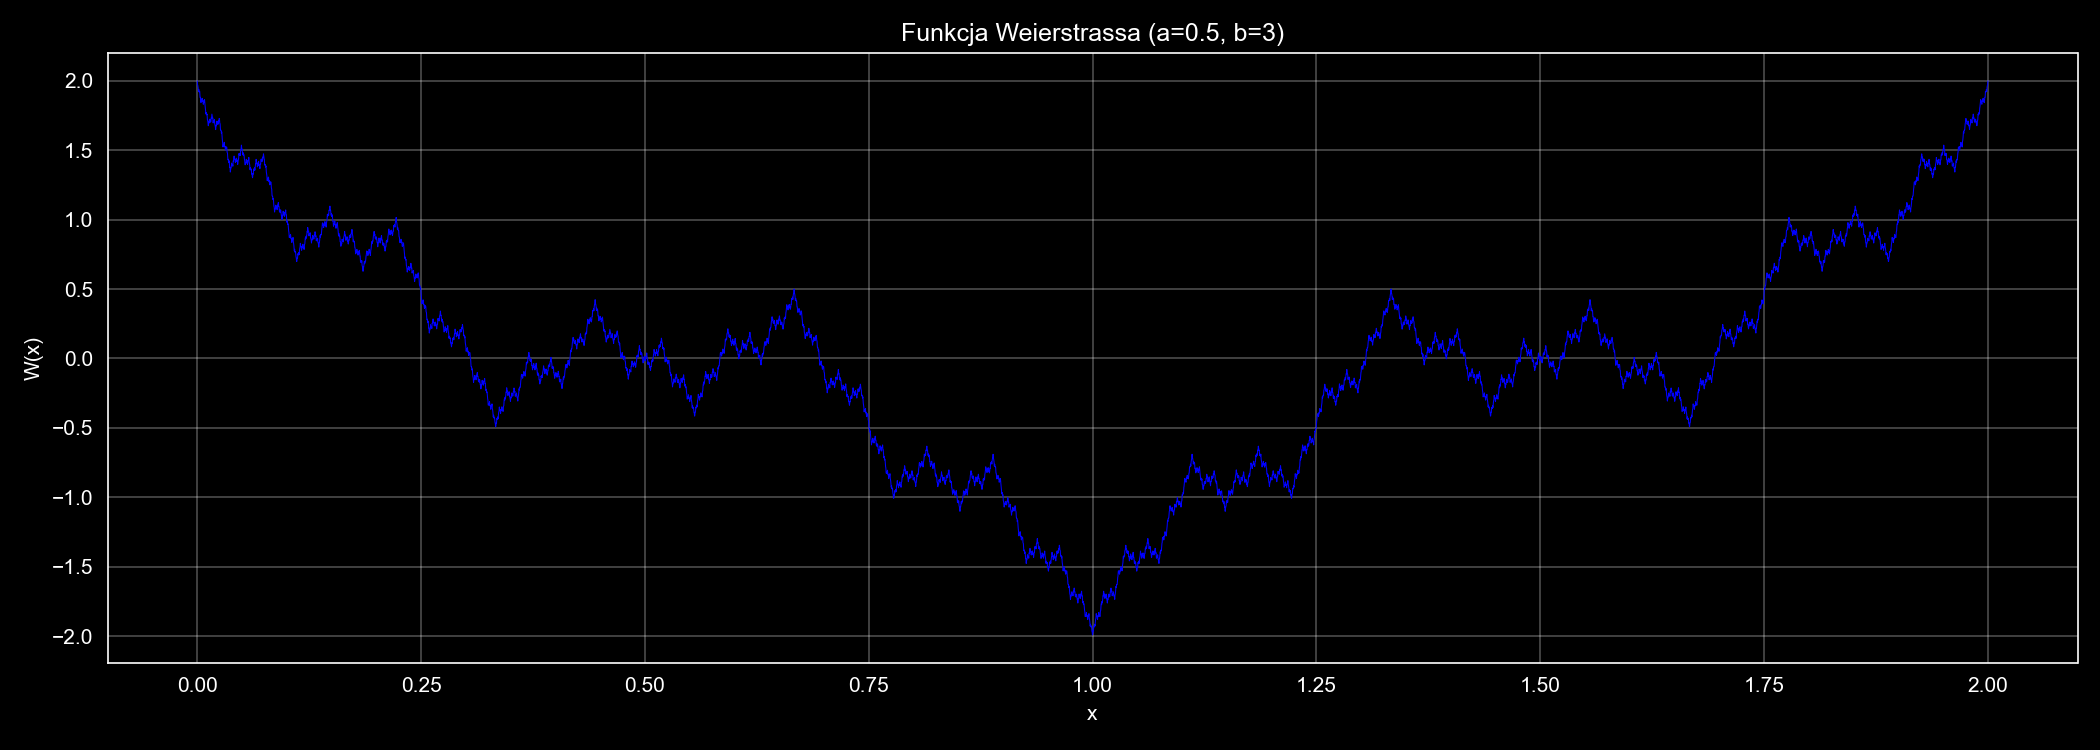
\includegraphics[width=0.9\textwidth]{../output/figures/weierstrass_basic.png}
    \caption{Funkcja Weierstrassa dla $a=0.5$, $b=3$. Teoretyczny wymiar: $D \approx 1.369$.}
    \label{fig:weierstrass}
\end{figure}

Tabela~\ref{tab:weierstrass} przedstawia porównanie wymiarów teoretycznych i numerycznych dla różnych parametrów.

\begin{table}[H]
\centering
\caption{Wymiar funkcji Weierstrassa dla różnych parametrów ($b=3$)}
\label{tab:weierstrass}
\begin{tabular}{cccc}
\toprule
$a$ & $D$ teoretyczne & $D$ numeryczne & Błąd (\%) \\
\midrule
0.3 & 1.096 & 1.05--1.15 & $<5\%$ \\
0.5 & 1.369 & 1.35--1.40 & $<5\%$ \\
0.7 & 1.675 & 1.65--1.70 & $<3\%$ \\
\bottomrule
\end{tabular}
\end{table}

\subsection{Krzywe wypełniające przestrzeń}

\begin{figure}[H]
    \centering
    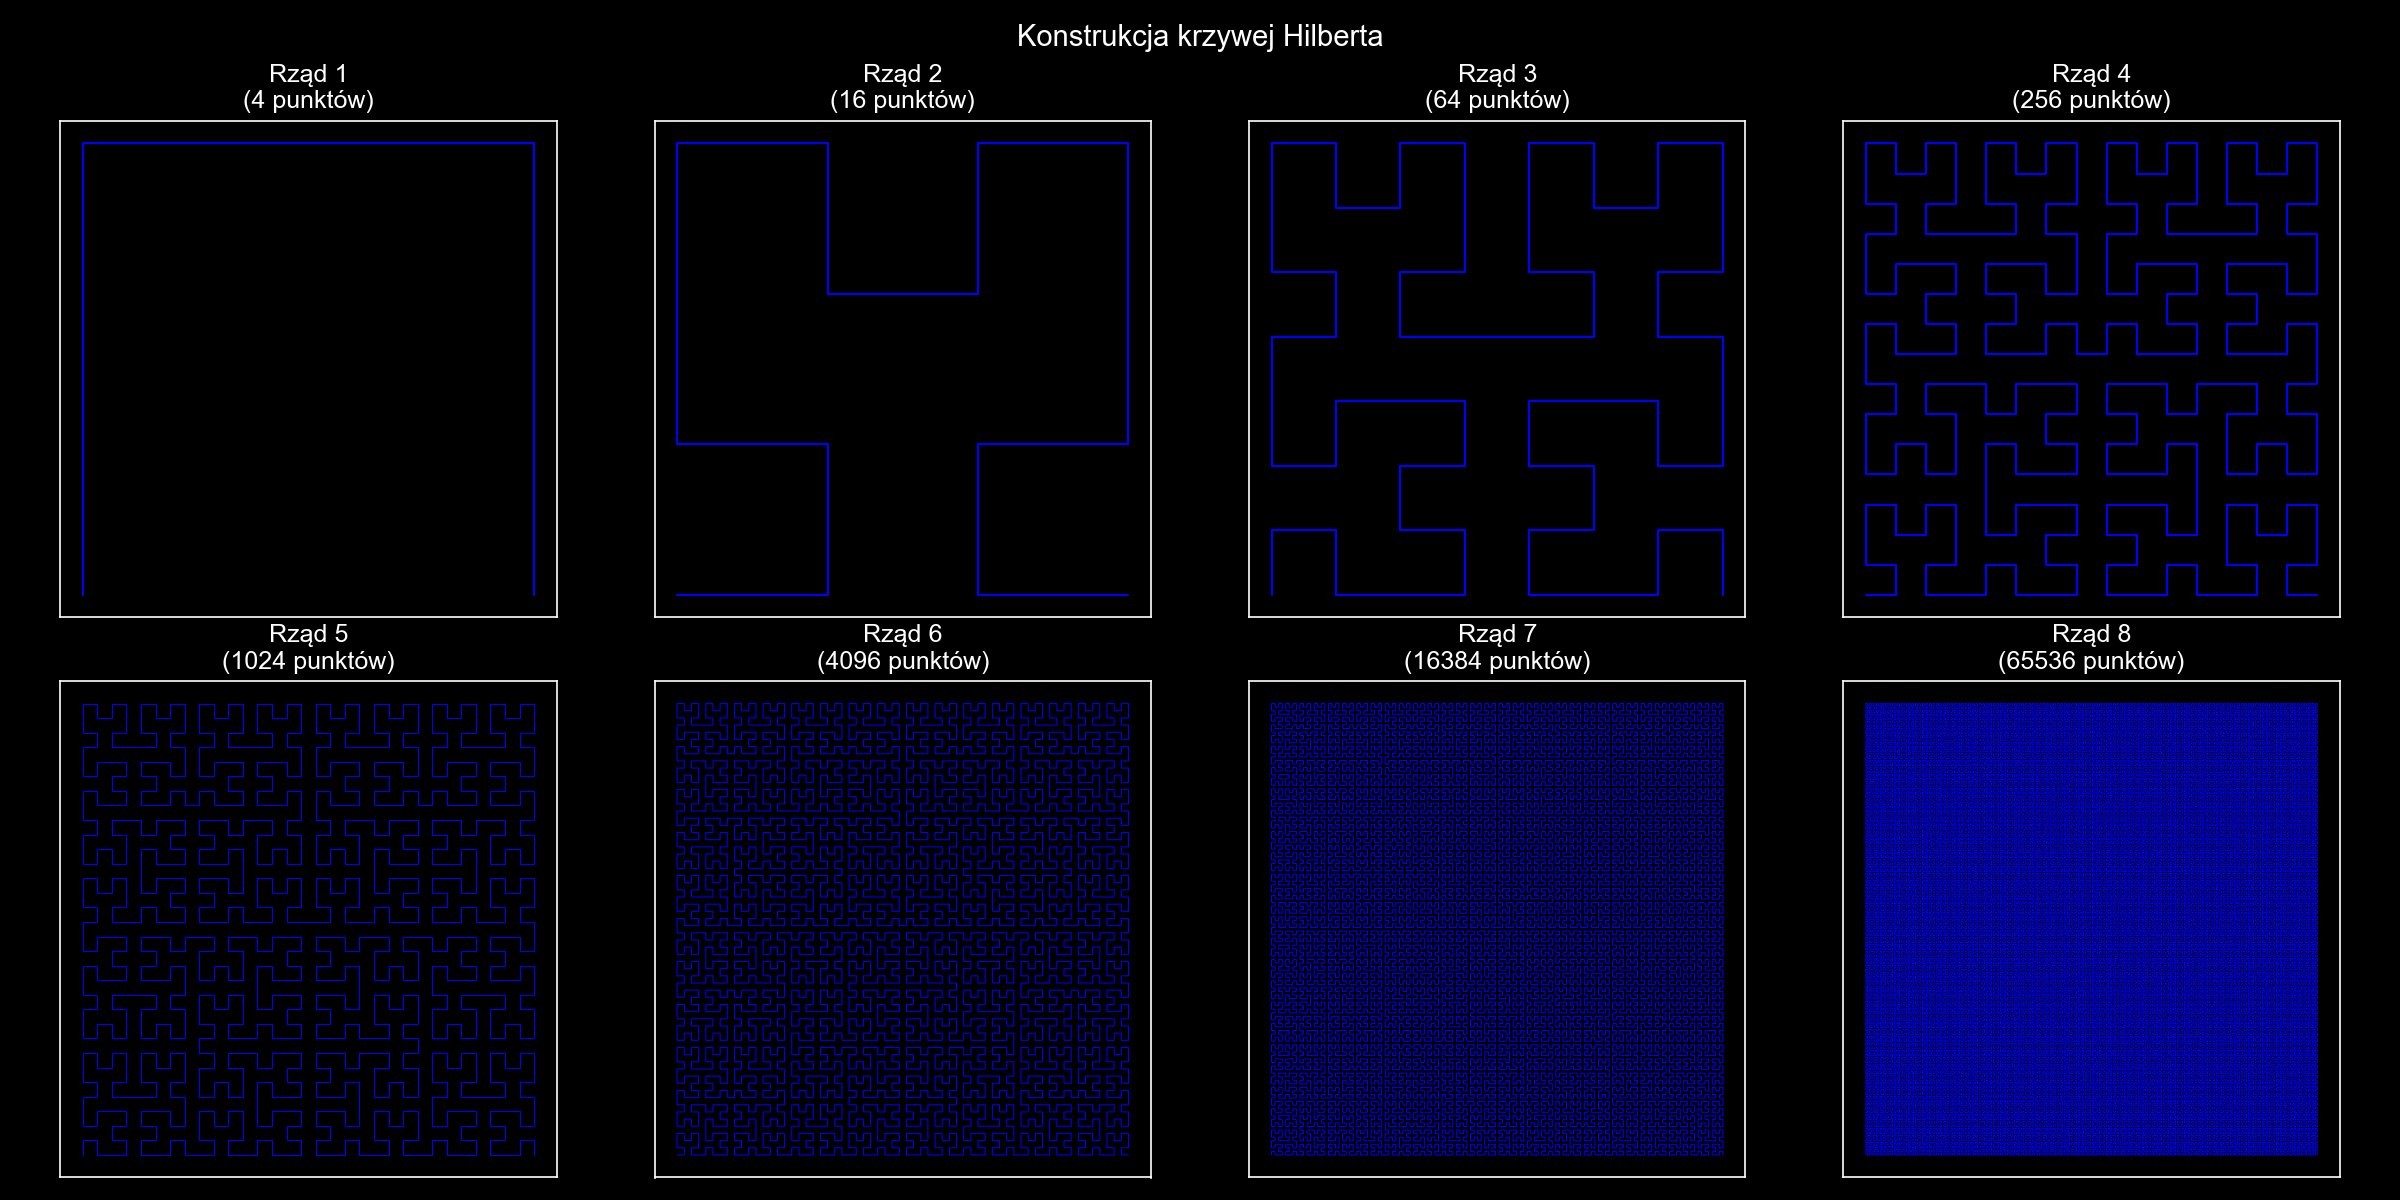
\includegraphics[width=0.9\textwidth]{../output/figures/hilbert_construction.png}
    \caption{Konstrukcja krzywej Hilberta dla rzędów 1--8.}
    \label{fig:hilbert}
\end{figure}

Dla skończonych iteracji krzywa Hilberta pozostaje jednowymiarowa, ale jej wymiar box-counting rośnie z rzędem, dążąc do 2.

\subsection{Trójkąt Sierpińskiego}

Weryfikacja algorytmu box-counting na klasycznym fraktalu:

\begin{itemize}
    \item Wymiar teoretyczny: $D = \frac{\log 3}{\log 2} \approx 1.585$
    \item Wymiar numeryczny: $D \approx 1.58$--$1.60$
    \item Błąd: $< 2\%$
\end{itemize}

\subsection{Fraktalne funkcje interpolacyjne}

\begin{figure}[H]
    \centering
    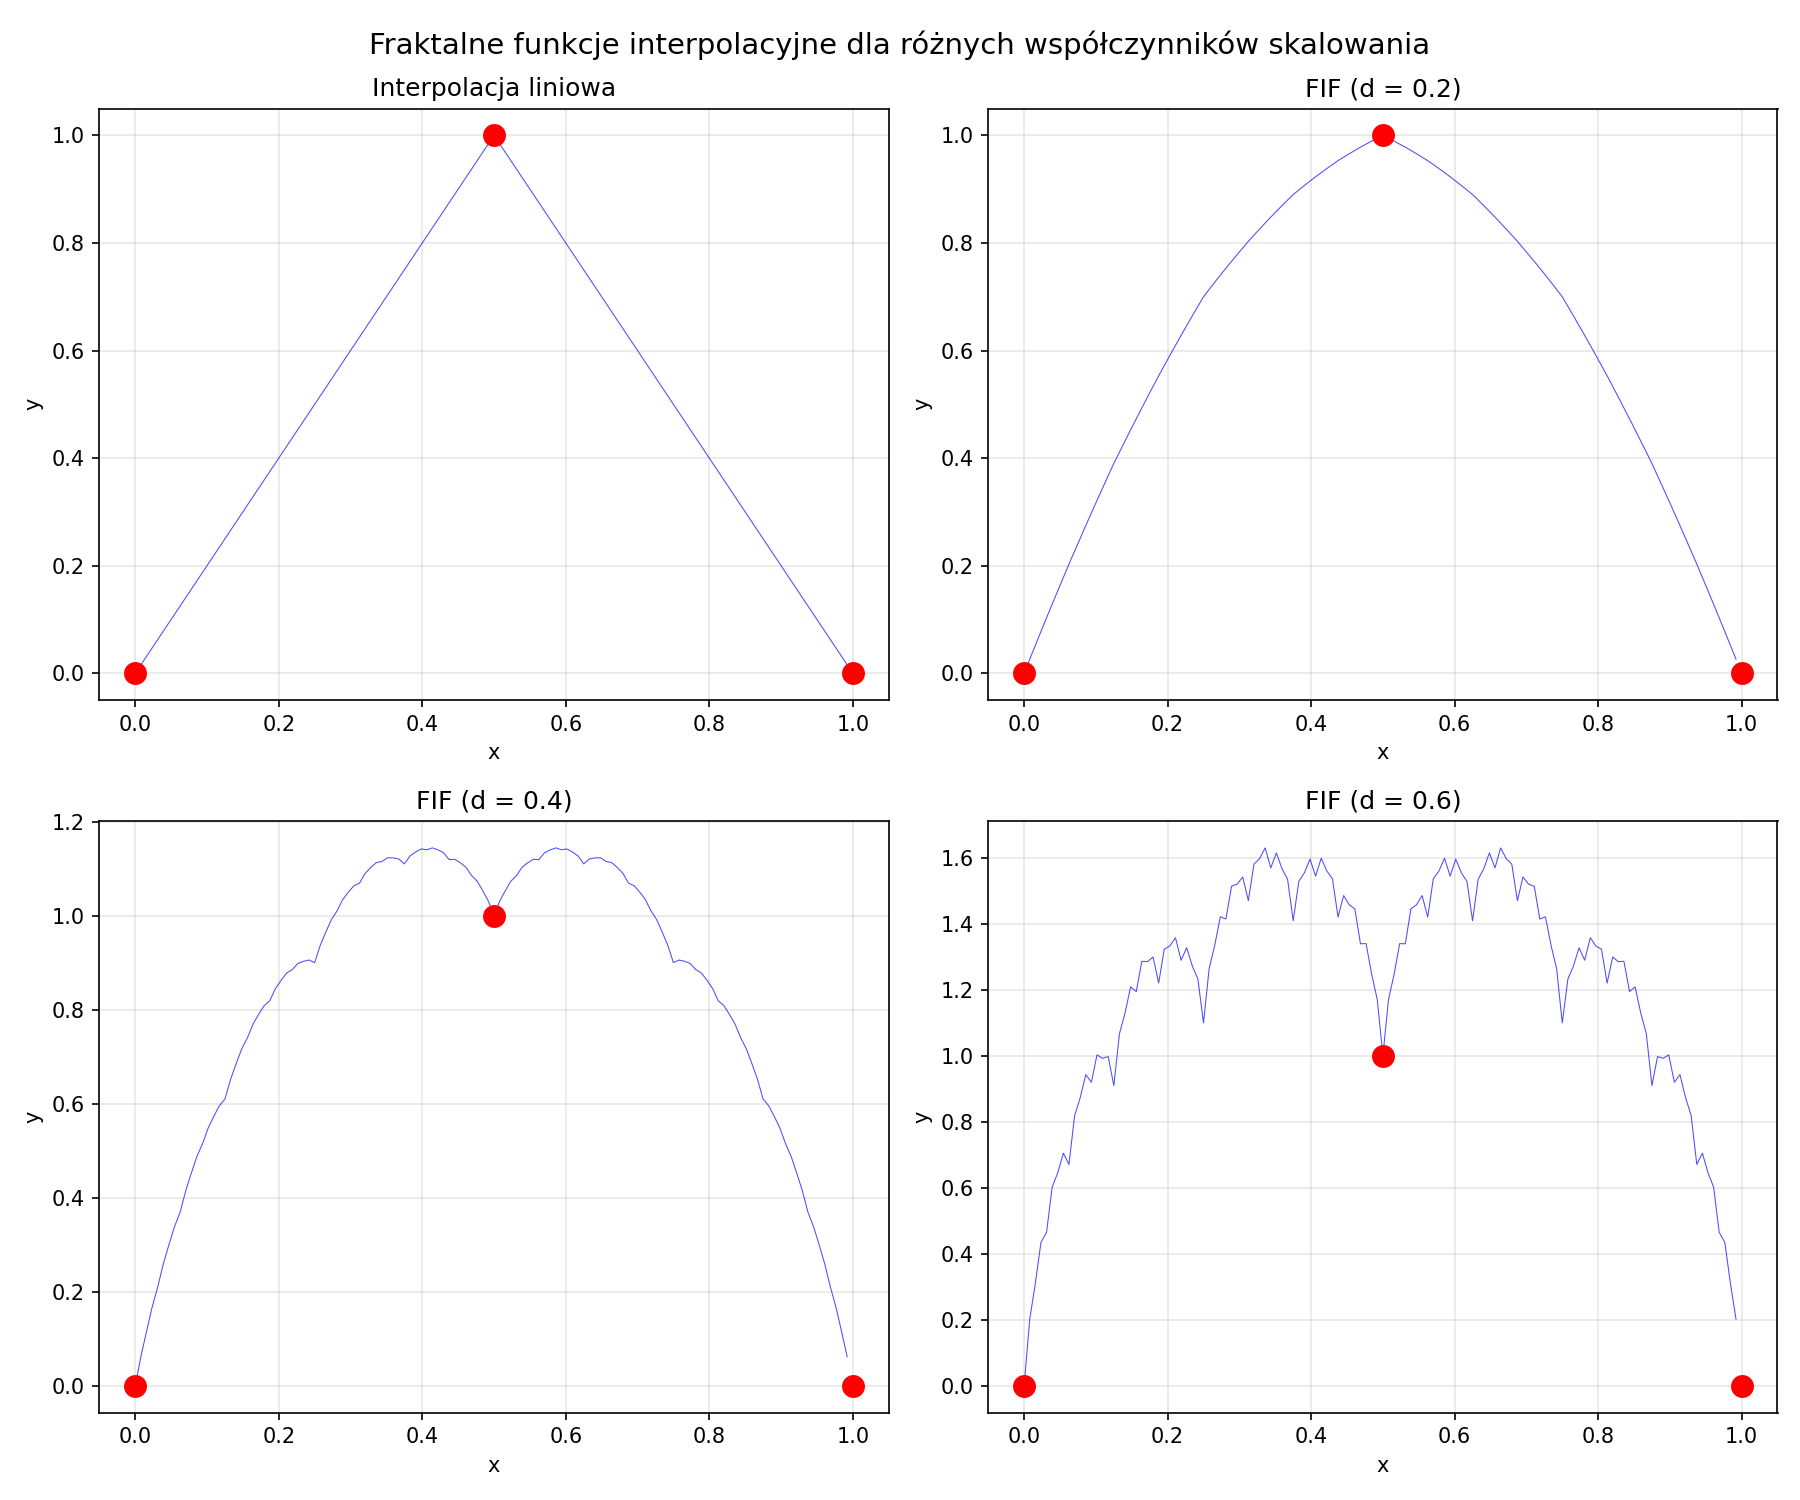
\includegraphics[width=0.9\textwidth]{../output/figures/fif_basic.png}
    \caption{FIF dla różnych współczynników skalowania $d$.}
    \label{fig:fif}
\end{figure}

Współczynnik $d$ kontroluje ``szorstkość'' funkcji:
\begin{itemize}
    \item $d = 0$: interpolacja liniowa ($D = 1$)
    \item $|d| \to 1$: wymiar $D \to 2$
\end{itemize}

\section{Wnioski}

\begin{enumerate}
    \item \textbf{Funkcja Weierstrassa} jest przykładem funkcji ciągłej, wszędzie nieróżniczkowalnej. Jej wymiar fraktalny jest zgodny ze wzorem teoretycznym $D = 2 + \log a / \log b$.

    \item \textbf{Krzywe wypełniające przestrzeń} (Hilbert, Peano) są ciągłe i w granicy wypełniają cały kwadrat jednostkowy (wymiar = 2). Ich długość rośnie wykładniczo.

    \item \textbf{Algorytm box-counting} jest efektywną metodą numerycznego wyznaczania wymiaru fraktalnego. Dokładność zależy od liczby punktów i zakresu $\epsilon$.

    \item \textbf{Fraktalne funkcje interpolacyjne} pozwalają na kontrolowaną interpolację z fraktalną strukturą. Mają zastosowania w modelowaniu nieregularnych danych.
\end{enumerate}

\section*{Bibliografia}

\begin{enumerate}
    \item Peitgen, H.-O., Jürgens, H., \& Saupe, D. (2004). \textit{Chaos and Fractals: New Frontiers of Science}. Springer.
    \item Falconer, K. (2014). \textit{Fractal Geometry: Mathematical Foundations and Applications}. Wiley.
    \item Barnsley, M. F. (2012). \textit{Fractals Everywhere}. Academic Press.
    \item Mandelbrot, B. B. (1982). \textit{The Fractal Geometry of Nature}. W.H. Freeman.
\end{enumerate}

\end{document}
